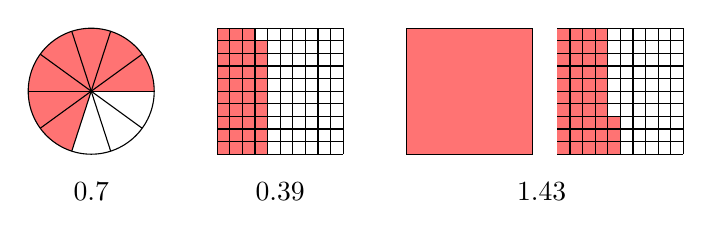
\begin{tikzpicture}[scale=.8]\fill[red!55](0,0)--(0:1)arc(0:252:1)--cycle;\draw(0,0)circle(1);\foreach\a in{0,36,...,324}\draw(0,0)--(\a:1);\node[below]at(0,-1.3){0.7};\begin{scope}[xshift=2cm]\foreach\i in{0,...,38}{\pgfmathtruncatemacro{\x}{floor(\i/10)}\pgfmathtruncatemacro{\y}{mod(\i,10)}\fill[red!55](\x*.2,\y*.2-1)rectangle(\x*.2+.2,\y*.2-.8);}\draw[step=.2](0,-1)grid(2,1);\node[below]at(1,-1.3){0.39};\end{scope}\begin{scope}[xshift=5cm]\fill[red!55](0,-1)rectangle(2,1);\draw(0,-1)rectangle(2,1);\foreach\i in{0,...,42}{\pgfmathtruncatemacro{\x}{floor(\i/10)}\pgfmathtruncatemacro{\y}{mod(\i,10)}\fill[red!55](\x*.2+2.4,\y*.2-1)rectangle(\x*.2+2.6,\y*.2-.8);}\draw[step=.2](2.4,-1)grid(4.4,1);\node[below]at(2.15,-1.3){1.43};\end{scope}\end{tikzpicture}
